\documentclass[mathserif]{beamer}
\usepackage{beamerthemeshadow}
\usepackage{beamerthemesplit}
%\usetheme{shadow}
\usecolortheme{default}
\setbeamertemplate{footline}[frame number]
\useinnertheme[shadow=true]{rounded}
%\setbeamertemplate{footline}{\insertframenumber/\inserttotalframenumber}
%\useoutertheme{infolines}
%\setbeamertemplate{headline}{} % removes the headline that infolines inserts

%\usetheme{boxes}
%\usepackage{amsmass}
%\usepackage{amssymb,amsfonts,url}


\usepackage{algorithm}
\usepackage{algorithmic}

\usepackage{graphicx}
\graphicspath{{Problems/}}
\usepackage{verbatim}

\usepackage{tikz}
\usetikzlibrary{shadows}
\usepackage{verbatim}
\usepackage{pgfplots}
\usepackage{verbatim}
\usetikzlibrary{arrows,shapes}

\definecolor{darkblue}{rgb}{0.2,0.2,0.6}
\definecolor{darkred}{rgb}{0.6,0.1,0.1}
\definecolor{darkgreen}{rgb}{0.2,0.6,0.2}

\usetikzlibrary{shadings,shadows,shapes.arrows}

\usetikzlibrary{calc} 

\tikzstyle{vertex}=[circle,fill=black!25,draw,minimum size=20pt,inner sep=0pt]
\tikzstyle{middlevertex}=[circle,fill=black!25,draw,minimum size=15pt,inner sep=0pt]
\tikzstyle{smallvertex}=[circle,fill=black!25,draw,minimum size=10pt,inner sep=0pt]
\tikzstyle{selected vertex} = [vertex, draw,fill=red!24]
\tikzstyle{blue smallvertex} = [smallvertex, draw,fill=blue]
\tikzstyle{red smallvertex} = [smallvertex, draw,fill=red]
\tikzstyle{edge} = [draw,thick,->]
\tikzstyle{undirectededge} = [draw,thick]
\tikzstyle{weight} = [font=\small]
\tikzstyle{selected edge} = [draw,line width=5pt,-,red!50]
\tikzstyle{ignored edge} = [draw,line width=5pt,-,black!20]

%\usepackage{CJK}
%\usepackage{pinyin}

%    \begin{figure}
%        \centering
%        \includegraphics[width=0.8\textwidth]{newGeneRep.eps}
%    \end{figure}

% \begin{figure}%
%   \begin{center}%
%     \begin{minipage}{0.70\textwidth}%
%      \includegraphics[width=1.0\textwidth]{comp25000.eps}%
%     \end{minipage}%
%     \begin{minipage}{0.30\textwidth}
%      \includegraphics[width=1.0\textwidth]{comparelabel.eps}%
%     \end{minipage}%
%   \end{center}
% \end{figure}

% \begin{table}
%   {\begin{tabular}{l|rrr}\hline
%       & \multicolumn{3}{c}{Actual number of DCJ operations}\\
%       \# genes &\# genes $\times 1$&\# genes $\times 2$&\# genes  $\times 3$ \\
% \hline
%      (a)~25,000 & 0.5\% ~~&  0.9\% ~~& 1.7\%~~\\
%       (b)~10,000 & 0.8\%~~ &  1.4\% ~~& 2.7\%~~\\
%      (c)~ 1,000 & 2.7\%~~ & 4.7\%~~ & 14.7\%~~\\ \hline
%     \end{tabular}} {}%
% \end{table}

% \begin{eqnarray}
% T(n) &=&  \sum_{i=1}^n C_i \\
%      &=&  \# PUSH + \#POP \\
%      &<& 2\times \#PUSH \\
%      &<& 2n \\
% \end{eqnarray}

% \[ 
% \begin{matrix}
% \begin{pmatrix}
% C_{11} & C_{12} \\ 
% C_{21} & C_{22} 
% \end{pmatrix}
% =
% \begin{pmatrix}
% A_{11} & A_{12} \\ 
% A_{21} & A_{22}  
% \end{pmatrix}
% 
% \begin{pmatrix}
% B_{11} & B_{12} \\ 
% B_{21} & B_{22}  
%  
% \end{pmatrix}
%     
%    \end{matrix}
% \]
% 
% 
% \begin{eqnarray}
%  C_{11} &=& (A_{11}\times B_{11}) + (A_{12} \times B_{21}) \\
% C_{12} &=& (A_{11}\times B_{12}) + (A_{12} \times B_{22}) \\
% C_{21} &=& (A_{21}\times B_{11}) + (A_{22} \times B_{21}) \\
% C_{22} &=& (A_{21}\times B_{12}) + (A_{22} \times B_{22}) 
% \end{eqnarray}
% \begin{figure}%
%      \begin{minipage}{0.32\textwidth}%
%       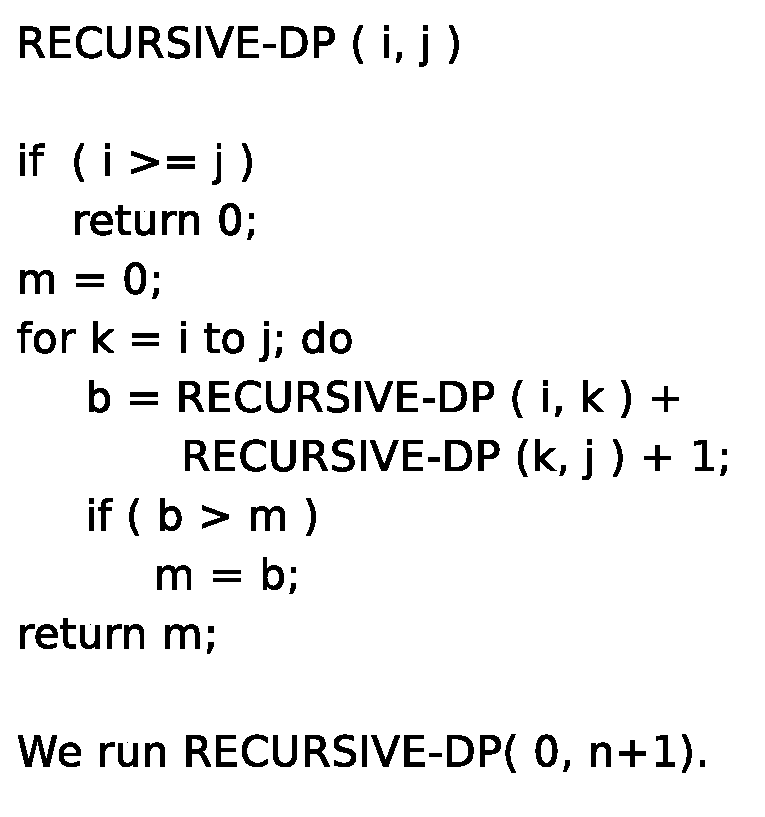
\includegraphics[width=1.0\textwidth]{L7-intervalschedulingdpalgo.eps}%
%      \end{minipage}%
%  \quad
%      \begin{minipage}{0.30\textwidth}
%       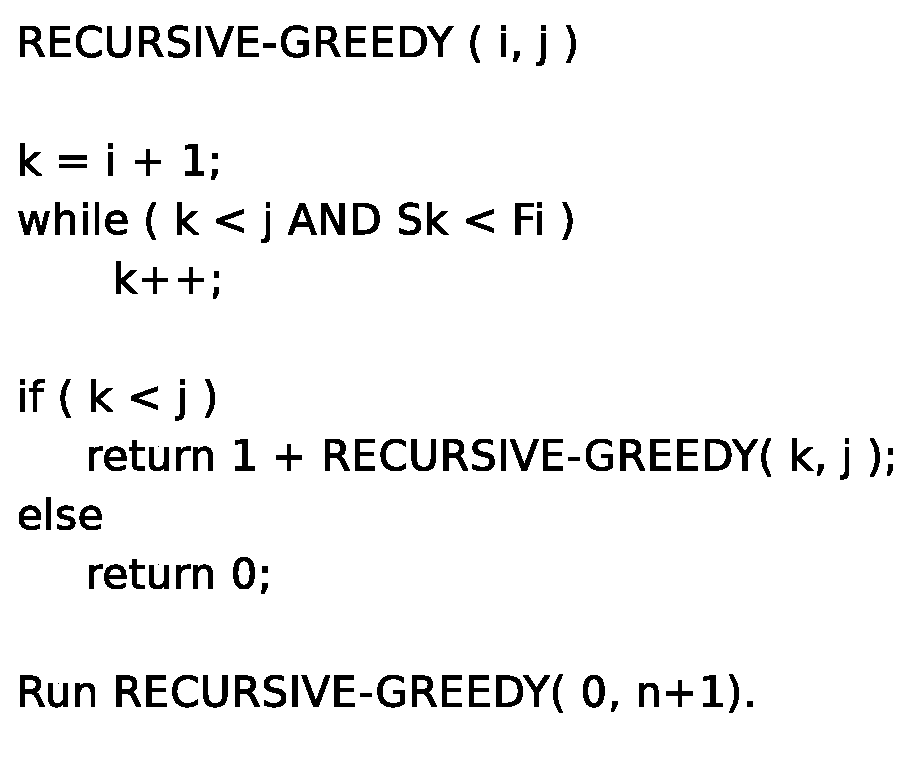
\includegraphics[width=1.0\textwidth]{L7-intervalschedulinggreedyalgo.eps}%
%      \end{minipage}%
%  \quad
%       \begin{minipage}{0.25\textwidth}
%       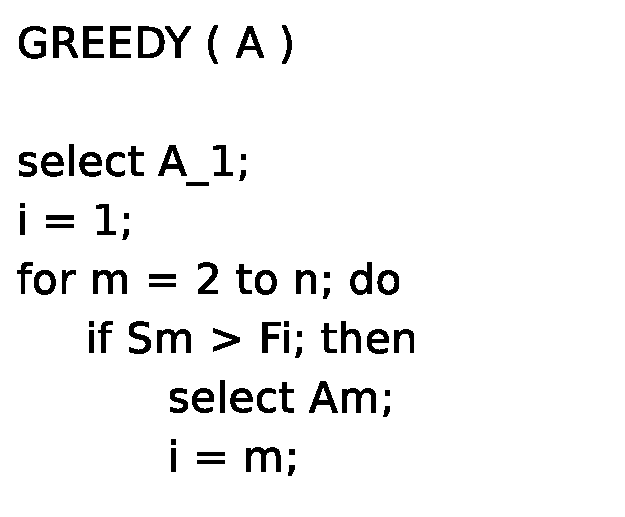
\includegraphics[width=1.0\textwidth]{L7-intervalschedulinggreedyalgo2.eps}%
%      \end{minipage}%
% 
%  \end{figure}

\title{CS711008Z  Algorithm Design and Analysis }
\subtitle{ Lecture 8.  Linear programming: interior point method
%\footnote{The slides were made based on Ch 29 of Introduction to algorithms, Combinatorial optimization algorithm and complexity by C. H. Papadimitriou and K. Steiglitz. } 
}
\author{Dongbo Bu } 
\institute{ {\small Institute of Computing Technology \\ 
Chinese Academy of Sciences, Beijing, China}}

\date{}
\begin{document}
%\begin{CJK}{UTF8}{cyberbit}
\frame{\titlepage}

\frame{
\frametitle{Outline}
\begin{itemize}
\item Brief history of interior point method
\item Basic idea of interior point method
\end{itemize}
} 


\frame{
\frametitle{A brief history of linear program}

\begin{itemize}
 \item In 1949, G. B. Dantzig proposed the simplex algorithm;
 \item In 1971, Klee and Minty gave a counter-example to show that simplex is not a polynomial-time algorithm.
 \item In 1975, L. V. Kantorovich and T. C. Koopmans, Nobel prize, application of linear programming in resource distribution;
 \item In 1979, L. G. Khanchian proposed a polynomial-time ellipsoid method;
 \item In 1984, N. Karmarkar proposed another polynomial-time interior-point method;
 \item In 2001, D. Spielman and S. Teng proposed smoothed complexity to prove the efficiency of simplex algorithm.
\end{itemize}
}


\frame{
	\frametitle{In 1979, L. G. Khanchian proposed a polynomial-time ellipsoid method for LP}
\begin{figure}
 \includegraphics[width=1.5in] {L8-Khachiyan.jpg}
\caption{Leonid G. Khanchian}
\end{figure}
}


\frame{
	\frametitle{In 1984, N. Karmarkar proposed a new polynomial-time algorithm for LP}
\begin{figure}
 \includegraphics[width=3in] {L8-Karmarkar.png}
 %\caption{In 1984, N. Karmarkar proposed a new polynomial-time algorithm for LP}
\end{figure}
}



\frame{
	\frametitle{}
	\begin{block}{}
	Basic idea of interior point method 
	\end{block}
} 

\frame{
	\frametitle{KKT conditions for LP}

\begin{itemize}
\item Let's consider a linear program in slack form and its dual problem, i.e. 
	\begin{itemize}
	\item 
Primal problem: 
\[
\begin{array}{rrrrrrrrl}
 \min & \mathnormal{ c^T x} &    & \\
 s.t. & \mathnormal{A x} &  \textcolor{red}{\mathnormal{= }} &  \mathnormal{b }     \\
      &\mathnormal{x} &  \textcolor{blue}{\mathnormal{\geq }}  & {0}\\
\end{array} \nonumber
\]

\item Dual problem: 
\[
\begin{array}{rrrrrrrl}
 \max & \mathnormal{b^T y} &     & \\
%s.t. & & & \\ 
% s.t. & \mathnormal{y}   & \textcolor{red}{\mathnormal{\geq }} & {0} \\
s.t.      & \mathnormal{A^T y} &  \textcolor{blue}{\mathnormal{\leq }} & \mathnormal{ c }   \\
\end{array} \nonumber
\]
	\end{itemize}
	\item KKT condition:   
		\begin{itemize}
			\item Primal feasibility: $Ax = b$, $x\geq 0$.
			\item Dual feasibility: $A^T y \leq c$
			\item Complementary slackness: $x_i = 0$, or $a_i^T y = c_i$ for any $i = 1, ..., m$.    
		\end{itemize}
%	\item Note that by this setting, complementary slackness follows as $\mathnormal{c^T x = c_B^T B^{-1} b =  y^T b }$. 
\end{itemize}


}

\frame{
	\frametitle{Rewriting KKT condition} 

\begin{itemize}
\item Let's consider a linear program in slack form and its dual problem, i.e. 
	\begin{itemize}
	\item 
Primal problem: 
\[
\begin{array}{rrrrrrrrl}
 \min & \mathnormal{ c^T x} &    & \\
 s.t. & \mathnormal{A x} &  \textcolor{red}{\mathnormal{= }} &  \mathnormal{b }     \\
      &\mathnormal{x} &  \textcolor{blue}{\mathnormal{\geq }}  & {0}\\
\end{array} \nonumber
\]

\item Dual problem: 
\[
\begin{array}{rrrrrrrl}
 \max & \mathnormal{b^T y} &     & \\
%s.t. & & & \\ 
% s.t. & \mathnormal{y}   & \textcolor{red}{\mathnormal{\geq }} & {0} \\
s.t.      & \mathnormal{A^T y} &  \textcolor{blue}{\mathnormal{\leq }} & \mathnormal{ c }   \\
\end{array} \nonumber
\]
	\end{itemize}
	\item KKT condition:   
		\begin{itemize}
			\item Primal feasibility: $Ax = b$, $x\geq 0$;
			\item Dual feasibility: $A^T y + \sigma = c$, $\sigma \geq 0$; 
			\item Complementary slackness: $x_i \sigma_i  = 0$.    
		\end{itemize}
		\item These conditions consists of $m+2n$ equations over $m+2n$ variables plus non-negative constraints. 
%	\item Note that by this setting, complementary slackness follows as $\mathnormal{c^T x = c_B^T B^{-1} b =  y^T b }$. 
\end{itemize}
	
}

\frame{
	\frametitle{Rewrite KKT conditions further} 
	
	\begin{itemize}
\item Let's define diagonal matrix: 
\[
X  =  \begin{matrix}
 \begin{pmatrix}
 x_1 & 0 & 0 \\
 0 & x_2 & 0 \\
 0 & 0 & x_3 
 \end{pmatrix}
 \end{matrix}, 
 \Sigma  =  \begin{matrix}
 \begin{pmatrix}
 \sigma_1 & 0 & 0 \\
 0 & \sigma_2 & 0 \\
 0 & 0 & \sigma_3 
 \end{pmatrix}
 \end{matrix}
\]
and rewrite the complementary slackness as: 
\[
X\Sigma e   =  \begin{matrix}
 \begin{pmatrix}
 x_1 \sigma_1 & 0 & 0 \\
 0 & x_2  \sigma_2& 0 \\
 0 & 0 & x_3 \sigma_3
 \end{pmatrix}
 \begin{pmatrix}
1\\
1\\
1
 \end{pmatrix}
= 
 \begin{pmatrix}
0\\
0\\
0
 \end{pmatrix}
 = 
 \begin{pmatrix}
x_1\sigma_1\\
x_2\sigma_2\\
x_3\sigma_3
 \end{pmatrix}

 \end{matrix}
\] 
	\item KKT condition:   
		\begin{itemize}
			\item Primal feasibility: $Ax = b$, $x\geq 0$;
			\item Dual feasibility: $A^T y + \sigma = c$, $\sigma \geq 0$; 
			\item Complementary slackness: $X \Sigma e   = 0$.    
		\end{itemize}
				\item We call $(x, y, \sigma)$  \textcolor{red}{\bf interior point} if $x>0$ and $\sigma>0$. 
				\item Question: How to find $(x, y, \sigma)$ satisfy the KKT conditions? 

%		\item These conditions consists of $m+2n$ equations over $m+2n$ variables plus non-negative constraints. 
%	\item Note that by this setting, complementary slackness follows as $\mathnormal{c^T x = c_B^T B^{-1} b =  y^T b }$. 
\end{itemize}
}


\frame{
	\frametitle{A simple interior-point method}
	\begin{itemize}
		\item Basic idea: Assume we have already known 
		$(\bar{x}, \bar{y}, \bar{\sigma})$ that are both primal and dual feasible, i.e., 
$A\bar{x} = b,  \bar{x} >  0$  
$ A^T \bar{y} + \bar{\sigma} = c, \bar{\sigma} > 0$ 

		and try to improve to another point $(x^*, y^*, \sigma^*)$ to make complementary slackness hold.   
		\item Improvement strategy:  Starting from $(\bar{x}, \bar{y}, \bar{\sigma})$, we follow a direction $(\Delta{x}, \Delta{y}, \Delta{\sigma})$ such that $(\bar{x}+\Delta{x}, \bar{y}+\Delta{y}, \bar{\sigma}+\Delta{\sigma})$ is a better solution, i.e., it comes closer to satisfying the complementary slackness. 
		\item To find such a direction, we substitute $(\bar{x}+\Delta{x}, \bar{y}+\Delta{y}, \bar{\sigma}+\Delta{\sigma})$ into the KKT conditions: 
		\begin{itemize}
			\item Primal feasibility: $A (\bar{x}+\Delta{x}) = b$, $\bar{x}+\Delta{x}\geq 0$;
			\item Dual feasibility: $A^T ( \bar{y}+\Delta{y} ) + (\bar{\sigma}+\Delta{\sigma}) = c$, $\bar{\sigma}+\Delta{\sigma}\geq 0$; 
			\item Complementary slackness: $(\bar{X}+\Delta{X}) (\bar{\Sigma}+\Delta{\Sigma}) e   = 0$.    
		\end{itemize}
	\end{itemize} 
}


\frame{
	\frametitle{}
	
	\begin{itemize}
		\item Since we start from $(\bar{x}, \bar{y}, \bar{\sigma})$ such that 
		$A\bar{x} = b,  \bar{x} >  0$  
$ A^T \bar{y} + \bar{\sigma} = c, \bar{\sigma} > 0$, the above conditions change into 
		\begin{itemize}
			\item $A \Delta{x} = 0$, $\bar{x}+\Delta{x}\geq 0$;
			\item  $A^T \Delta{y} + \Delta{\sigma} = 0$, $\bar{\sigma}+\Delta{\sigma}\geq 0$; 
			\item $\bar{X}\Delta{\sigma} +  \bar{\Sigma}\Delta{x} = - \bar{X} \bar{\Sigma} e - \Delta{X} \Delta{\Sigma} e  
			$.    
		\end{itemize}
		\item Let's apply the Newton's method to solve these nonlinear equations. Note that when $\Delta x$ and $\Delta \sigma$ are small, the final non-linear term $- \Delta{X} \Delta{\Sigma} e$ is small relative to $ - \bar{X} \bar{\Sigma} e$ and can thus be dropped out, generating a linear system. 
		\begin{itemize}
			\item $A \Delta{x} = 0$, $\bar{x}+\Delta{x}\geq 0$;
			\item  $A^T \Delta{y} + \Delta{\sigma} = 0$, $\bar{\sigma}+\Delta{\sigma}\geq 0$; 
			\item $\bar{X}\Delta{\sigma} +  \bar{\Sigma}\Delta{x} = - \bar{X} \bar{\Sigma} e  
			$    
		\end{itemize}
		\item The solution are: 
		$\Delta \sigma = \bar{X}^{-1}(- \bar{X}\bar{\Sigma} - \bar{\Sigma}\Delta x  ) = -\bar{\sigma} -   \bar{X}^{-1}\bar{\Sigma} \Delta x$ 
\[
\begin{matrix}
 \begin{pmatrix}
 - \bar{X}^{-1}\bar{\Sigma} & A^T \\
A & 0 
 \end{pmatrix}
 \begin{pmatrix}
\Delta x \\
\Delta y
 \end{pmatrix}
= 
 \begin{pmatrix}
\bar{\sigma}\\
0
 \end{pmatrix}
 \end{matrix}
\] 		 
	\end{itemize}
 
}


\frame{

        
\begin{algorithmic}[1]
\begin{small}
\STATE Set initial solution $\bar{x}$ such that $A\bar{x} = b$, $\bar{x}>0$; 
\STATE Set initial solution $\bar{y}, \bar{\sigma}$ such that $A^T\bar{y} + \bar{\sigma} = c$, $\bar{\sigma}>0$; 
\WHILE{\texttt{TRUE}}       
 	\STATE Solve 
\[
\begin{matrix}
 \begin{pmatrix}
 - \bar{X}^{-1}\bar{\Sigma} & A^T \\
A & 0 
 \end{pmatrix}
 \begin{pmatrix}
\Delta x \\
\Delta y
 \end{pmatrix}
= 
 \begin{pmatrix}
\bar{\sigma}\\
0
 \end{pmatrix}
 \end{matrix}
\]
\STATE Set $\Delta \sigma = \bar{X}^{-1}(- \bar{X}\bar{\Sigma} - \bar{\Sigma}\Delta x  ) = -\bar{\sigma} -   \bar{X}^{-1}\bar{\Sigma} \Delta x$; 
\STATE Set $\theta_x = \min_{j: \Delta x_j < 0} \frac{\bar{x_j}}{-\Delta x_j}$, $\theta_\sigma = \min_{j: \Delta \sigma_j < 0} \frac{\bar{\sigma_j}}{-\Delta \sigma_j }$; 
\STATE Set  $\theta = \min\{1, \alpha \theta_x, \alpha \theta_\sigma\}$; 
 \STATE Update $\bar{x} = \bar{x} + \theta \Delta{x}$, $\bar{y} = \bar{y} + \theta \Delta{y}$, $\bar{\sigma} = \bar{\sigma} + \theta \Delta{\sigma}$; 
 		 
\IF{$x_i \sigma_i \leq \epsilon$  for all $i = 1, ..., m$}                 
	\STATE break;
        \ENDIF
\ENDWHILE
\RETURN $(x, y, \sigma)$;
\end{small}
\end{algorithmic}
}


\frame{
	\frametitle{An example}
	
	\[
\begin{array}{rrrrrrrrrrrrl}
 \min & 2x_1    &+ 1.5x_2   &      &     \\
   s.t.  &12x_1       &+24 x_2           & \geq & 120  \\
%     &             & y_2      & \leq & 0  \\
  &16x_1       &+16 x_2           & \geq & 120  \\
  &30x_1       &+12 x_2           & \geq & 120  \\
     &   x_1          &       & \leq & 15  \\
     &             & x_2      & \leq & 15  \\
     &   x_1          &       & \geq & 0  \\
     &             & x_2      & \geq & 0  
     \end{array} \nonumber
\]
} 

%\frame{ 
%	\frametitle{An execution}
%
%\begin{itemize}	
%	\item Starting point 1: $x = (10, 10)$.
%	\item Starting point 2: $x = (14, 1)$.
%
%\begin{figure}
%	\includegraphics[width=3in]{IPM1.png}
%\end{figure}
%
%\end{itemize}
%
%}

\frame{ 
	\frametitle{An execution}

\begin{itemize}	
	\item Starting point 1: $x = (10, 10)$.
\end{itemize}	

	\begin{figure}[H]
	\center
	\begin{tikzpicture}[scale=0.4, auto,swap]
	\draw[black, fill=green!10] (15, 15) -- (0, 15) -- (0, 10) -- (1.667, 5.833) -- (5, 2.5) -- (10, 0) -- (15, 0) --  cycle;
	\draw[->] (-0.5, -0.5) -- (16, -0.5) node[below] {$x_1$};
	\draw[->] (-0.5, -0.5) -- (-0.5, 16) node[left] {$x_2$};  
	\foreach \x/\xtext in { 0/0, 5/5, 10/10, 15/15 }
		\draw[gray,shift={(\x, -0.5)}] (0pt,3pt) -- (0pt,0pt) node[black, below] {\tiny $\xtext$};
	\foreach \y/\ytext in { 0/0, 5/5, 10/10, 15/15 }
		\draw[gray,shift={(-0.5, \y)}] (3pt,0pt) -- (0pt,0pt) node[black, left] {\tiny $\ytext$}; 

\draw[red, fill=red] (10.000000, 10.000000) circle (3pt);
\draw[red, fill=red] (9.900797, 9.935846) circle (3pt);
\draw[red, fill=red] (6.989100, 9.224929) circle (3pt);
\draw[red, fill=red] (3.242048, 8.542336) circle (3pt);
\draw[red, fill=red] (1.983477, 6.619660) circle (3pt);
\draw[red, fill=red] (2.026596, 5.478920) circle (3pt);
\draw[red, fill=red] (1.876891, 5.623137) circle (3pt);
\draw[red, fill=red] (1.720388, 5.779612) circle (3pt);
\draw[red, fill=red] (1.668339, 5.831661) circle (3pt);

	\end{tikzpicture}
\end{figure}


}


\frame{ 
	\frametitle{Another execution}

\begin{itemize}	
	\item Starting point 2: $x = (14, 1)$.
\end{itemize}	
	\begin{figure}[H]
	\center
	\begin{tikzpicture}[scale=0.4, auto,swap]
	\draw[black, fill=green!10] (15, 15) -- (0, 15) -- (0, 10) -- (1.667, 5.833) -- (5, 2.5) -- (10, 0) -- (15, 0) --  cycle;
	\draw[->] (-0.5, -0.5) -- (16, -0.5) node[below] {$x_1$};
	\draw[->] (-0.5, -0.5) -- (-0.5, 16) node[left] {$x_2$};  
	\foreach \x/\xtext in { 0/0, 5/5, 10/10, 15/15 }
		\draw[gray,shift={(\x, -0.5)}] (0pt,3pt) -- (0pt,0pt) node[black, below] {\tiny $\xtext$};
	\foreach \y/\ytext in { 0/0, 5/5, 10/10, 15/15 }
		\draw[gray,shift={(-0.5, \y)}] (3pt,0pt) -- (0pt,0pt) node[black, left] {\tiny $\ytext$}; 




\draw[red, fill=red] (14.000000, 1.000000) circle (3pt);
\draw[red, fill=red] (13.391962, 0.751488) circle (3pt);
\draw[red, fill=red] (11.996010, 0.710194) circle (3pt);
\draw[red, fill=red] (9.734954, 0.653762) circle (3pt);
\draw[red, fill=red] (8.622182, 0.691515) circle (3pt);
\draw[red, fill=red] (8.178611, 0.910707) circle (3pt);
\draw[red, fill=red] (6.946300, 1.526854) circle (3pt);
\draw[red, fill=red] (5.009725, 2.495140) circle (3pt);
\draw[red, fill=red] (5.000042, 2.499982) circle (3pt);
\draw[red, fill=red] (4.999992, 2.500008) circle (3pt);
\draw[red, fill=red] (4.999987, 2.500014) circle (3pt);
\draw[red, fill=red] (4.999973, 2.500027) circle (3pt);
\draw[red, fill=red] (4.999946, 2.500054) circle (3pt);
\draw[red, fill=red] (4.999893, 2.500107) circle (3pt);
\draw[red, fill=red] (4.999786, 2.500214) circle (3pt);
\draw[red, fill=red] (4.999574, 2.500426) circle (3pt);
\draw[red, fill=red] (4.999149, 2.500851) circle (3pt);
\draw[red, fill=red] (4.998303, 2.501697) circle (3pt);
\draw[red, fill=red] (4.996615, 2.503385) circle (3pt);
\draw[red, fill=red] (4.993249, 2.506751) circle (3pt);
\draw[red, fill=red] (4.986541, 2.513459) circle (3pt);
\draw[red, fill=red] (4.973185, 2.526815) circle (3pt);
\draw[red, fill=red] (4.946645, 2.553355) circle (3pt);
\draw[red, fill=red] (4.894110, 2.605890) circle (3pt);
\draw[red, fill=red] (4.790935, 2.709065) circle (3pt);
\draw[red, fill=red] (4.591460, 2.908540) circle (3pt);
\draw[red, fill=red] (4.217783, 3.282217) circle (3pt);
\draw[red, fill=red] (3.561226, 3.938774) circle (3pt);
\draw[red, fill=red] (2.552111, 4.947889) circle (3pt);
\draw[red, fill=red] (1.671094, 5.828906) circle (3pt);
\draw[red, fill=red] (1.666689, 5.833311) circle (3pt);
\draw[red, fill=red] (1.666667, 5.833333) circle (3pt);
\draw[red, fill=red] (1.666667, 5.833333) circle (3pt);
\draw[red, fill=red] (1.666667, 5.833333) circle (3pt);
\draw[red, fill=red] (1.666667, 5.833333) circle (3pt);
	\end{tikzpicture}
\end{figure}


}





\frame{
	\frametitle{Centered interior-point method}
	\begin{itemize}
		\item To avoid the poor performance, we need a way to keep the iterate away from the boundary until the solution approaches the optimum. 
		\item An efficient way to achieve this goal is to relax complementary slackness: 
\[
	X \Sigma e   = 0
\]
into 
\[
	X \Sigma e   =  \mu e \quad (\mu >0) 
\]
	\item We start from a large $\mu$, and gradually  reduce it as the algorithm proceeds. At each iteration, we execute the previous affine interior point method.  
		
	\end{itemize}

}


\frame{

        
\begin{algorithmic}[1]
\begin{small}
\STATE Set initial solution $\bar{x}$ such that $A\bar{x} = b$, $\bar{x}>0$; 
\STATE Set initial solution $\bar{y}, \bar{\sigma}$ such that $A^T\bar{y} + \bar{\sigma} = c$, $\bar{\sigma}>0$; 
\WHILE{\texttt{TRUE}}       
	\STATE \textcolor{red}{Estimate $\bar{\mu} = \beta \frac{\bar{\sigma}\bar{x}}{n}$};  
 	\STATE Solve 
\[
\begin{matrix}
 \begin{pmatrix}
 - \bar{X}^{-1}\bar{\Sigma} & A^T \\
A & 0 
 \end{pmatrix}
 \begin{pmatrix}
\Delta x \\
\Delta y
 \end{pmatrix}
= 
 \begin{pmatrix}
\bar{\sigma}  \textcolor{red}{-\bar{\mu} \bar{X}^{-1} e}\\
0
 \end{pmatrix}
 \end{matrix}
\]
\STATE Set $\Delta \sigma = \bar{X}^{-1}(- \bar{X}\bar{\Sigma} - \bar{\Sigma}\Delta x  ) = -\bar{\sigma} -   \bar{X}^{-1}( \bar{\Sigma} \Delta x \textcolor{red}{-\bar{\mu}e } $); 
\STATE Set $\theta_x = \min_{j: \Delta x_j < 0} \frac{\bar{x_j}}{-\Delta x_j}$, $\theta_\sigma = \min_{j: \Delta \sigma_j < 0} \frac{\bar{\sigma_j}}{-\Delta \sigma_j }$; 
\STATE Set  $\theta = \min\{1, \alpha \theta_x, \alpha \theta_\sigma\}$; 
 \STATE Update $\bar{x} = \bar{x} + \theta \Delta{x}$, $\bar{y} = \bar{y} + \theta \Delta{y}$, $\bar{\sigma} = \bar{\sigma} + \theta \Delta{\sigma}$; 
 		 
\IF{$x_i \sigma_i \leq \epsilon$  for all $i = 1, ..., m$}                 
	\STATE break;
        \ENDIF
\ENDWHILE
\RETURN $(x, y, \sigma)$;
\end{small}
\end{algorithmic}
}



\frame{ 
	\frametitle{Running center path algorithm} 

\begin{itemize}	
	\item Starting point 1: $x = (10, 10)$.
\end{itemize}	

	\begin{figure}[H]
	\center
	\begin{tikzpicture}[scale=0.4, auto,swap]
	\draw[black, fill=green!10] (15, 15) -- (0, 15) -- (0, 10) -- (1.667, 5.833) -- (5, 2.5) -- (10, 0) -- (15, 0) --  cycle;
	\draw[->] (-0.5, -0.5) -- (16, -0.5) node[below] {$x_1$};
	\draw[->] (-0.5, -0.5) -- (-0.5, 16) node[left] {$x_2$};  
	\foreach \x/\xtext in { 0/0, 5/5, 10/10, 15/15 }
		\draw[gray,shift={(\x, -0.5)}] (0pt,3pt) -- (0pt,0pt) node[black, below] {\tiny $\xtext$};
	\foreach \y/\ytext in { 0/0, 5/5, 10/10, 15/15 }
		\draw[gray,shift={(-0.5, \y)}] (3pt,0pt) -- (0pt,0pt) node[black, left] {\tiny $\ytext$}; 



\draw[blue, fill=red] (10.000000, 10.000000) circle (3pt);
\draw[blue, fill=red] (10.830319, 10.768231) circle (3pt);
\draw[blue, fill=red] (11.105872, 11.051477) circle (3pt);
\draw[blue, fill=red] (11.129017, 11.093152) circle (3pt);
\draw[blue, fill=red] (11.050500, 11.045635) circle (3pt);
\draw[blue, fill=red] (10.899111, 10.943751) circle (3pt);
\draw[blue, fill=red] (10.660758, 10.785361) circle (3pt);
\draw[blue, fill=red] (10.294019, 10.551653) circle (3pt);
\draw[blue, fill=red] (9.727703, 10.213430) circle (3pt);
\draw[blue, fill=red] (8.861775, 9.740202) circle (3pt);
\draw[blue, fill=red] (7.623965, 9.125954) circle (3pt);
\draw[blue, fill=red] (6.151841, 8.415829) circle (3pt);
\draw[blue, fill=red] (4.834045, 7.676068) circle (3pt);
\draw[blue, fill=red] (3.880823, 6.985352) circle (3pt);
\draw[blue, fill=red] (3.237070, 6.434402) circle (3pt);
\draw[blue, fill=red] (2.809401, 6.054113) circle (3pt);
\draw[blue, fill=red] (2.522189, 5.824399) circle (3pt);
\draw[blue, fill=red] (2.314297, 5.716484) circle (3pt);
\draw[blue, fill=red] (2.147899, 5.694692) circle (3pt);
\draw[blue, fill=red] (2.013150, 5.714696) circle (3pt);
\draw[blue, fill=red] (1.910914, 5.743509) circle (3pt);
\draw[blue, fill=red] (1.837501, 5.768295) circle (3pt);
\draw[blue, fill=red] (1.785918, 5.787060) circle (3pt);
\draw[blue, fill=red] (1.749896, 5.800677) circle (3pt);
\draw[blue, fill=red] (1.724777, 5.810379) circle (3pt);
\draw[blue, fill=red] (1.707261, 5.817230) circle (3pt);
\draw[blue, fill=red] (1.695039, 5.822048) circle (3pt);
\draw[blue, fill=red] (1.686504, 5.825428) circle (3pt);
\draw[blue, fill=red] (1.680541, 5.827798) circle (3pt);
\draw[blue, fill=red] (1.676373, 5.829458) circle (3pt);
\draw[blue, fill=red] (1.673458, 5.830620) circle (3pt);
\draw[blue, fill=red] (1.671419, 5.831434) circle (3pt);
\draw[blue, fill=red] (1.669993, 5.832004) circle (3pt);
\draw[blue, fill=red] (1.668995, 5.832403) circle (3pt);
\draw[blue, fill=red] (1.668296, 5.832682) circle (3pt);
\draw[blue, fill=red] (1.667807, 5.832877) circle (3pt);

	\end{tikzpicture}
\end{figure}

}

\frame{ 
	\frametitle{Running center path algorithm} 

\begin{itemize}	
	\item Starting point 2: $x = (14, 1)$.
\end{itemize}	

	\begin{figure}[H]
	\center
	\begin{tikzpicture}[scale=0.4, auto,swap]
	\draw[black, fill=green!10] (15, 15) -- (0, 15) -- (0, 10) -- (1.667, 5.833) -- (5, 2.5) -- (10, 0) -- (15, 0) --  cycle;
	\draw[->] (-0.5, -0.5) -- (16, -0.5) node[below] {$x_1$};
	\draw[->] (-0.5, -0.5) -- (-0.5, 16) node[left] {$x_2$};  
	\foreach \x/\xtext in { 0/0, 5/5, 10/10, 15/15 }
		\draw[gray,shift={(\x, -0.5)}] (0pt,3pt) -- (0pt,0pt) node[black, below] {\tiny $\xtext$};
	\foreach \y/\ytext in { 0/0, 5/5, 10/10, 15/15 }
		\draw[gray,shift={(-0.5, \y)}] (3pt,0pt) -- (0pt,0pt) node[black, left] {\tiny $\ytext$}; 


%\draw[blue, fill=blue] (14.000000, 1.000000) circle (3pt);
%\draw[blue, fill=blue] (11.934509, 1.757599) circle (3pt);
%\draw[blue, fill=blue] (4.541888, 3.195373) circle (3pt);
%\draw[blue, fill=blue] (3.908869, 3.958304) circle (3pt);
%\draw[blue, fill=blue] (1.776171, 5.944078) circle (3pt);
%\draw[blue, fill=blue] (1.692294, 5.873723) circle (3pt);
%\draw[blue, fill=blue] (1.697185, 5.820065) circle (3pt);
%\draw[blue, fill=blue] (1.675828, 5.829573) circle (3pt);
%\draw[blue, fill=blue] (1.669404, 5.832237) circle (3pt);
%\draw[blue, fill=blue] (1.667489, 5.833004) circle (3pt);

\draw[blue, fill=blue] (14.000000, 1.000000) circle (3pt);
\draw[blue, fill=blue] (10.928171, 3.494093) circle (3pt);
\draw[blue, fill=blue] (8.054184, 8.766748) circle (3pt);
\draw[blue, fill=blue] (5.904430, 8.239339) circle (3pt);
\draw[blue, fill=blue] (5.457101, 7.945094) circle (3pt);
\draw[blue, fill=blue] (4.732375, 7.546629) circle (3pt);
\draw[blue, fill=blue] (4.134014, 7.135876) circle (3pt);
\draw[blue, fill=blue] (3.656629, 6.765200) circle (3pt);
\draw[blue, fill=blue] (3.279706, 6.452810) circle (3pt);
\draw[blue, fill=blue] (2.984712, 6.202204) circle (3pt);
\draw[blue, fill=blue] (2.754018, 6.010750) circle (3pt);
\draw[blue, fill=blue] (2.571264, 5.873454) circle (3pt);
\draw[blue, fill=blue] (2.422373, 5.783998) circle (3pt);
\draw[blue, fill=blue] (2.296922, 5.734236) circle (3pt);
\draw[blue, fill=blue] (2.188798, 5.714137) circle (3pt);
\draw[blue, fill=blue] (2.095352, 5.713295) circle (3pt);
\draw[blue, fill=blue] (2.015591, 5.722956) circle (3pt);
\draw[blue, fill=blue] (1.948712, 5.737040) circle (3pt);
\draw[blue, fill=blue] (1.893539, 5.751969) circle (3pt);
\draw[blue, fill=blue] (1.848580, 5.765935) circle (3pt);
\draw[blue, fill=blue] (1.812252, 5.778197) circle (3pt);
\draw[blue, fill=blue] (1.783055, 5.788585) circle (3pt);
\draw[blue, fill=blue] (1.759665, 5.797200) circle (3pt);
\draw[blue, fill=blue] (1.740961, 5.804251) circle (3pt);
\draw[blue, fill=blue] (1.726019, 5.809975) circle (3pt);
\draw[blue, fill=blue] (1.714087, 5.814598) circle (3pt);
\draw[blue, fill=blue] (1.704559, 5.818319) circle (3pt);
\draw[blue, fill=blue] (1.696950, 5.821308) circle (3pt);
\draw[blue, fill=blue] (1.690873, 5.823706) circle (3pt);
\draw[blue, fill=blue] (1.686018, 5.825627) circle (3pt);
\draw[blue, fill=blue] (1.682138, 5.827166) circle (3pt);
\draw[blue, fill=blue] (1.679038, 5.828398) circle (3pt);
\draw[blue, fill=blue] (1.676560, 5.829385) circle (3pt);
\draw[blue, fill=blue] (1.674579, 5.830174) circle (3pt);
\draw[blue, fill=blue] (1.672995, 5.830806) circle (3pt);
\draw[blue, fill=blue] (1.671728, 5.831311) circle (3pt);
\draw[blue, fill=blue] (1.670715, 5.831715) circle (3pt);
\draw[blue, fill=blue] (1.669905, 5.832039) circle (3pt);
\draw[blue, fill=blue] (1.669257, 5.832298) circle (3pt);
\draw[blue, fill=blue] (1.668739, 5.832505) circle (3pt);
\draw[blue, fill=blue] (1.668324, 5.832671) circle (3pt);
\draw[blue, fill=blue] (1.667993, 5.832803) circle (3pt);



	\end{tikzpicture}
\end{figure}


}


\frame{
	\frametitle{Find the optimum $x^*$ when setting $\mu=0.01, 0.1, 0.5, 1$} 
	
		\begin{figure}
%		\includegraphics[width=4in]{L8-logbarrier2.png}
		\includegraphics[width=2in]{L8-IPM-t100.png}
		\includegraphics[width=2in]{L8-IPM-t10.png}
%		\includegraphics[width=2in]{L8-IPM-t5.png}
		\includegraphics[width=2in]{L8-IPM-t2.png}
		\includegraphics[width=2in]{L8-IPM-t1.png}
	\end{figure}
 	
}


\frame{
	\frametitle{Another viewpoint }
	
	\begin{itemize}
		\item Actually, the relaxed complementary slackness 
\[
	X \Sigma e   =  \tfrac{1}{t} e \quad (t >0) 
\]
		corresponds to the following constrained optimization problem: 
	\[
\begin{array}{rrrlllrrrrl}
 \min & \mathnormal{ c^T x} &-& \frac{1}{t} \sum\limits_{i=1}^n \log x_i  \\
 s.t. & \mathnormal{A x}  &\textcolor{red}{\mathnormal{= }} &  \mathnormal{b }    \\
      &\mathnormal{x}  & \textcolor{blue}{\mathnormal{\geq }} &  {0} \\
\end{array} \nonumber
\]
	
		
	\end{itemize}

}




\frame{
\frametitle{Consider a general optimization problem}

\begin{itemize}
	\item Suppose we are trying to solve a convex program with \textcolor{red}{\bf inequality constraints}: 
	
	\[
\begin{array}{rrrrrrrrrrrrl}
 \min & f({x})   \\
 s.t. & \mathnormal{Ax = b} \\
      & \textcolor{red}{g({x}) \leq 0} \\
\end{array} \nonumber
\]

 where $f({x})$ and  $g({x})$ are convex, and twice differentiable. 

\end{itemize}


} 



\frame{
\frametitle{Let's start from \textcolor{red}{\bf equality constrained} quadratic programming} 

\begin{itemize}
	\item Suppose we are trying to solve a QP with \textcolor{red}{\bf equality constraints} : 
	
	\[
\begin{array}{ccccccc}
 \min & \frac{1}{2} {x}^T \mathnormal{P x + Q}^T \mathnormal{x + r }     \\
 s.t. & \mathnormal{Ax = b} \\
%      & g({x}) \leq 0 \\
\end{array} \nonumber
\]
\item Applying Lagrangian conditions, we have \\
\begin{center}
	 $\mathnormal{Ax^* = b}$, and 
	 $\mathnormal{P x^* + Q} +  \mathnormal{A^T \lambda } = 0 $
	 \end{center}
	  
\item Thus, the optimum point $\mathnormal{x^*}$ can be solved as follows: 

\begin{center}

$ \left[\begin{array}{cc} \mathnormal{P} & \mathnormal{A^T} \\ \mathnormal{A} & \mathnormal{0}\end{array}\right]    \left[\begin{array}{c} \mathnormal{x^*}  \\ \mathnormal{\lambda} \end{array}\right] =   \left[\begin{array}{c} -\mathnormal{Q}  \\ \mathnormal{b} \end{array}\right]$

\end{center}

\end{itemize}

} 


\frame{
\frametitle{Then how to minimize  $f({x})$  with \textcolor{red}{\bf equality constraints}? Newton's method}

\begin{itemize}
	\item Suppose we are trying to minimize a convex function $f({x})$, which is not a QP. 
	\[
\begin{array}{rrrrrrrrrrrrl}
 \min & f({x})   \\
 s.t. & \mathnormal{Ax = b} \\
%      & \textcolor{red}{g({x}) \leq 0} \\
\end{array} \nonumber
\]
	\item Basic idea: let's try to improve from a feasible solution ${x}$. At ${x}$, we write the Taylor extension, and use \textcolor{red}{\bf quadratic approximation} to $\tilde{f}({x + \Delta x }) = f({x })  + \bigtriangledown f({x} )  + \frac{1}{2} \Delta { x}^T \bigtriangledown^2 f({x}) \Delta{x} $
		\[
\begin{array}{rrrrrrrrrrrrl}
 \min &  \tilde{f}({x+\Delta x})      \\
 s.t. & \mathnormal{A (x + \Delta x) = b} \\
%      & \textcolor{red}{g({x}) \leq 0} \\
\end{array} \nonumber
\]
	  
\item Thus, the optimum point $\Delta \mathnormal{ x^*}$ can be solved as follows: 

\begin{center}

$ \left[\begin{array}{cc} \mathnormal{\bigtriangledown^2}f({x}) & \mathnormal{A^T} \\ \mathnormal{A} & \mathnormal{0}\end{array}\right]    \left[\begin{array}{c} \Delta \mathnormal{ x^*}  \\ \mathnormal{\lambda} \end{array}\right] =   \left[\begin{array}{c} - \bigtriangledown f({x})  \\ \mathnormal{b} \end{array}\right]$

\end{center}
\item Since this is just an approximation to $f(x)$, we need to iteratively perform line search. 

\end{itemize}

} 



\frame{
\frametitle{Then how to minimize  $f({x})$  with \textcolor{red}{\bf inequality constraints}? }
\begin{itemize}
	\item Suppose we are trying to solve a convex program with \textcolor{red}{\bf inequality constraints}: 
	
	\[
\begin{array}{rrrrrrrrrrrrl}
 \min & f({x})   \\
 s.t. & \mathnormal{Ax = b} \\
      & \textcolor{red}{g({x}) \leq 0} \\
\end{array} \nonumber
\]

 where $f({x})$ and  $g({x})$ are convex, and twice differentiable. 

\item Basic idea: 
	\begin{enumerate}
		\item Transform it into a series of \textcolor{red}{\bf equality constrainted} optimisation problems; 
		\item Solve each \textcolor{red}{\bf equality constrainted} optimisation problem using Newton's method. 
	\end{enumerate}

\end{itemize}


} 


\frame{
	\begin{block}{}
		Log barrier function: transform into \textcolor{red}{\bf equality constraints} 
	\end{block}

}

\frame{
	\frametitle{Log barrier function }
\begin{itemize}
	\item Suppose we are trying to solve a convex program with \textcolor{red}{\bf inequality constraints}: 
	
	\[
\begin{array}{rrrrrrrrrrrrl}
 \min & f({x})   \\
 s.t. & \mathnormal{Ax = b} \\
      & \textcolor{red}{g({x}) \leq 0} \\
\end{array} \nonumber
\]

 where $f({x})$ and  $g({x})$ are convex, and twice differentiable. 
\item This is equivalent to the following optimization problem. 

	\[
\begin{array}{rrrrrrrrrrrrl}
 \min & f({x})  + \textcolor{red}{ I\_(g({x})) }   \\
 s.t. & \mathnormal{Ax = b} \\
%      & \textcolor{red}{g({x}) \leq 0} \\
\end{array} \nonumber
\]

where  $I\_(u)  = \begin{cases} 0 & \text{ if }  u \leq 0 \\ \infty & \text{ otherwise}  \end{cases}$

\item But indicator function is not differentiable. 
\end{itemize} 	
} 	


\frame{
	\frametitle{Log barrier function: \textcolor{red}{\bf smooth approximation} to the indicator function}
\begin{itemize}
	\item Suppose we are trying to solve a convex program with \textcolor{red}{\bf inequality constraints}: 
	
	\[
\begin{array}{rrrrrrrrrrrrl}
 \min & f({x})   \\
 s.t. & \mathnormal{Ax = b} \\
      & \textcolor{red}{g({x}) \leq 0} \\
\end{array} \nonumber
\]

 where $f({x})$ and  $g({x})$ are convex, and twice differentiable. 
\item This is equivalent to the following optimization problem. 

	\[
\begin{array}{rrrrrrrrrrrrl}
 \min & f({x})   \textcolor{red}{ - \frac{1}{t} \log( - g({x})) }   \\
 s.t. & \mathnormal{Ax = b} \\
%      & \textcolor{red}{g({x}) \leq 0} \\
\end{array} \nonumber
\]
\item Basic idea: a smooth approximation to indicator function 
$\textcolor{red}{ -\frac{1}{t} \log( -u)} $, and this approximation improves as $t\rightarrow \infty$. 

\end{itemize} 	
} 	



\frame{
	\frametitle{Log barrier function approximates indicator function} 
	
%	\begin{figure}
%		\includegraphics[width=3in]{L8-logbarrier.png}
%	\end{figure}

\begin{figure}
\begin{tikzpicture}[x=1.0cm,y=1.0cm,scale=0.85] 
%\pgfplotsset{my style/.append style={ axis x line=middle, axis y line=middle, axis equal }}

    \begin{axis}[anchor=origin,         xlabel=$u$,
        ylabel=$ $, 
        xtick={ -2,..., 2},
        ytick={ -5, 0, 5, 10}, 
        xmin=-2.5,
        xmax=2.5,
        ymin=-5,
        ymax=10, 
         x=1cm, y=0.25cm, 
        ];
	
              \addplot[domain=-3:-0.00001, red, thick]{ -1.0/0.8* ln(-x)};
%              \addplot[domain=-2.5:2.5, green, ultra thick]{1*x};
%              \addplot[domain=-1:3,-,red]{-x+1};	
      \end{axis};
      
      	\def\dy{0};
	\draw[blue, ultra thick] (-2.5, 0+\dy) -- (0, 0+\dy); 
	\draw[dashed, blue, ultra thick] (0, 0+\dy) -- (0, 2.5+\dy); 

	\node[blue, ultra thick] at (0.8, 1.8) {$I_{-}(u)$};

        \node[red, ultra thick] at (-1.2, 1.6) {$-\frac{1}{t} \log(-u)$};
        \node[red, ultra thick] at (-1.2, 1.0) {$(t > 0)$};

%        \node[green, ultra thick] at (0.8, -0.5) {$-\lambda u$ $(\lambda < 0)$};

%              \node[red] at (4,0) {$x_3+x_4=1$};
%	\draw[fill=blue] (0, 0) -- ( 2, 0) -- (4,3) -- (0,1) -- (0,05);
%	\node[circle, minimum size=3pt,inner sep=0pt, fill=red] at (0,0) {};
%		\node[circle, minimum size=3pt,inner sep=0pt, fill=red] at (2,0) {};
%			\node[circle, minimum size=3pt,inner sep=0pt, fill=red] at (4,3) {};
%			\node[below, red, ultra thick] at (-0.2,-0.2) {start};
%			\node[below, red, ultra thick] at (4.2,3) {end};	
%			\draw[->, red, ultra thick] (0,0) -- (2,0); 
%			\draw[->, red, ultra thick] (2,0) -- (4,3); 
			
    \end{tikzpicture}
\end{figure}


\begin{itemize}
\item 
$\textcolor{red}{ -\frac{1}{t} \log( -u)} $ approximates the indicator function, and the approximation improves as $t\rightarrow \infty$. 
\item For each setting of $t$, we obtain an approximation to the original optimisation problem. 
\end{itemize}

}


\frame{
	\frametitle{Interior method and central path} 
	
\begin{itemize}
	\item Solve a sequence of optimization problem: 
		\[
\begin{array}{rrrrrrrrrrrrl}
 \min & f({x})   \textcolor{red}{ - \frac{1}{t} \log( - g({x})) }   \\
 s.t. & \mathnormal{Ax = b} \\
%      & \textcolor{red}{g({x}) \leq 0} \\
\end{array} \nonumber
\]
	\item For any $t > 0$, we define $x^{*}(t)$ as the optimal solution.
	\item $t$ increases step by step.  $t$ should not be too large initially, as it is not easy to solve it using Newton's method. 
	\item Central path: $\{x^{*}(t) | t > 0 \}$. 
	\end{itemize}
}

 \frame{
 	\frametitle{Interior point method for LP}
	
	\begin{itemize}
		\item Consider the following LP 
		\[
\begin{array}{rrrrrrrrrrrrl}
 \min & \mathnormal{c^Tx} &   &\\
 s.t. & \mathnormal{Ax} &\leq & b \\
      & \mathnormal{x} &\geq & 0 \\
\end{array} \nonumber
\]
	\end{itemize}
 
	\begin{figure}
		\includegraphics[width=4in]{L8-logbarrier2.png}
%		\includegraphics[width=4in]{L8-logbarrier3.png}
	\end{figure}
 	
 } 
 
 
 \frame{
	\frametitle{Central path} 
	
\begin{itemize}
	\item For any $t>0$,  we define $x^{*}(t)$ as the optimal solution  to:
			\[
\begin{array}{rrrrrrrrrrrrl}
 \min & f({x})   \textcolor{red}{ - \frac{1}{t} \log( - g({x})) }   \\
 s.t. & \mathnormal{Ax = b} \\
%      & \textcolor{red}{g({x}) \leq 0} \\
\end{array} \nonumber
\]
	\item $x^{*}(t)$ is not optimal solution to the original problem. 
	\item The duality gap is bounded by $\frac{m}{t}$. 
\end{itemize}
}

 
 \frame{
 	\frametitle{Interior point algorithm }
	
	\begin{figure}
		\includegraphics[width=4in]{L8-logbarrier4.png}
	\end{figure}
	
		
} 	
 

\end{document}
